\documentclass[9pt]{book}

% This line takes a 6x9 page and futzes with the margins to make it
% look right inside a bound book.
\usepackage[centering,width=4.5in,height=7.5in,includeall,twoside,hcentering,vcentering,marginparsep=0in,marginparwidth=0in]{geometry}

\usepackage{dogecoin-tricks_commands}
\usepackage[OnyxNeon]{onfancy}
\usepackage{onyxneon}
\usepackage[english]{babel}
\usepackage{graphicx}

\DefineVerbatimEnvironment{CodeListing}{Verbatim}{gobble=2,fontfamily=courier,commandchars=\\\{\},fontsize=\footnotesize}
\DefineVerbatimEnvironment{programlisting}{Verbatim}{gobble=2,fontfamily=courier,commandchars=\\\{\},fontsize=\scriptsize}
\DefineVerbatimEnvironment{Screen}{Verbatim}{gobble=0,fontfamily=courier,commandchars=\\\{\},fontsize=\footnotesize}

\newcommand*{\dogebreak}{
    \nottoggle{isFirstSectionInChapter} { 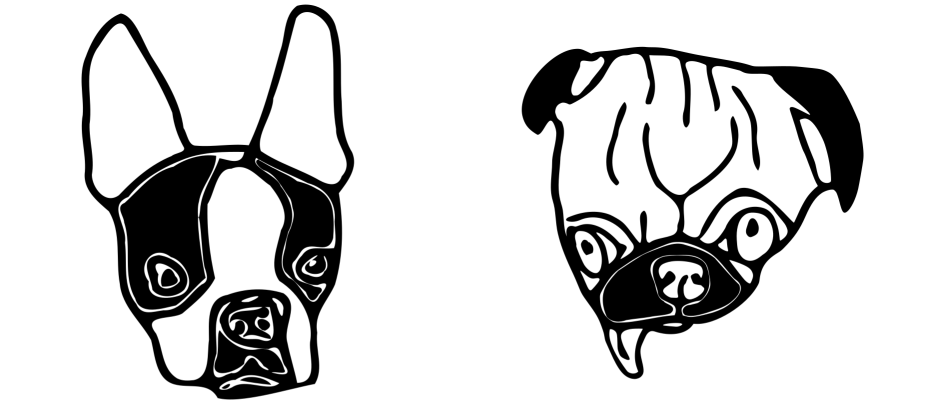
\includegraphics[height=2em]{Dogebreak.png} } {} %
}

\newcommand*{\dogesectionbreak}{
    \par %
%    \begin{center} $\dogebreak\ \ \ \dogebreak\ \ \ \dogebreak\ \ \ $ \end{center} %
}

\titleformat{\section}
{}
{\filright 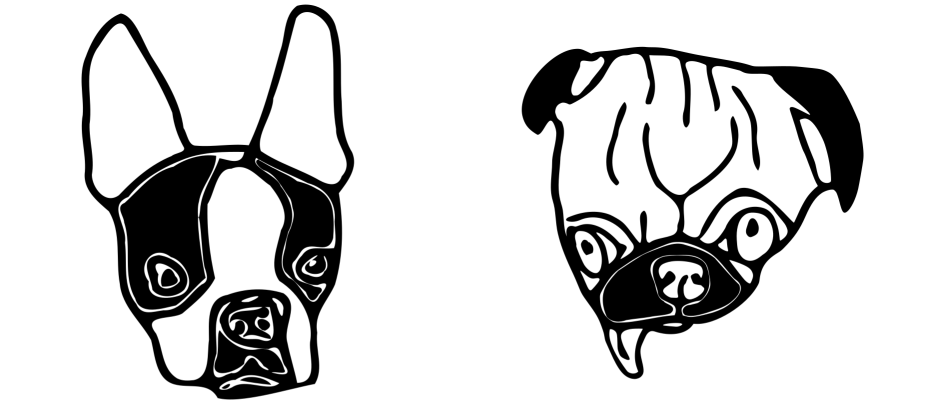
\includegraphics[height=2em]{Dogebreak.png} \Large\bfseries \enspace Tip \#\arabic{tipsCounter}\enspace }
{8pt}
{\Large\bfseries}
[\vspace{2ex}\titlerule\vspace{2ex}]

% \newcommand{\sectionbreak}{\nopagebreak[4] \begin{center} $\dogebreak\ \ \ \dogebreak\ \ \ \dogebreak\ \ \ $ \end{center}}

% start sections on new pages
% \newcommand{\sectionbreak}{\clearpage}

\makeindex

\usepackage{titletoc}
\usepackage[firstpageonly=true]{draftwatermark}

\usepackage{ifthen}

\begin{document}
\belowdisplayskip=0pt

% suppress section numbering but include A-heads in ToC
\setcounter{tocdepth}{1}
\setcounter{secnumdepth}{3}

\addtolength{\parskip}{3pt}
\addtolength{\skip\footins}{10pt}
\addtolength{\footnotesep}{5pt}
% \headline={\hrulefill}
% \footline={\hrulefill}

% this could become the \bookfrontmatter command
\frontmatter
\pagestyle{empty}
\maketitle
\thispagestyle{empty}

\huge{\booktitle}
\newline
\large{\booksubtitle}
\newline
\newline
\normalsize

Copyright \copyright~2024 \bookauthor

\vfill
\textbf{Editor:} \bookauthor\newline
\textbf{Cover design:} Natalie Wood

% \textbf{ISBN-10:} \bookisbnten\newline
\textbf{ISBN-13:} \bookisbnthirteen

This book uses the Onyx Neon toolset. See \url{https://onyxneon.com/} for more
details.

Onyx Neon typesets books with free software, especially Linux, Perl, PseudoPod,
and \LaTeX. Many thanks to the contributors who make these and other projects
possible.

First edition November 2024.

For more details, see \url{https://ifdogethenwow.com/books/dogecoin-tricks/}.
Please \emph{do} share this link with your friends and colleagues.

Thanks for reading!

\thispagestyle{empty}
\clearpage
\begin{center}
    \thispagestyle{empty}
    \vspace*{\fill}
    \em{For Rosie}

    April 26, 2024

    8:52 pm
    \vspace*{\fill}
\end{center}
\clearpage

\addtocontents{toc}{\protect\thispagestyle{empty}}
\tableofcontents
\clearpage
% mark foreword and preface specially
\pagestyle{fancy}
\addcontentsline{toc}{chapter}{Foreword}
\fancyhead[OR]{\nouppercase {\em Foreword}}
\pagenumbering{roman}
\include{chapter_foreword}
\addcontentsline{toc}{chapter}{Preface}
\fancyhead[OR]{\nouppercase {\em Preface}}
\include{chapter_00}
\thispagestyle{empty}

\mainmatter

% and now the rest
\fancyhead[OR]{\nouppercase {\em \leftmark}}
\setcounter{secnumdepth}{2}

% set a global counter
\newcounter{tipsCounter}
\AddToHook{cmd/section/before}{\stepcounter{tipsCounter}}
\renewcommand\thesection{\#\arabic{tipsCounter}}

\providetoggle{isFirstSectionInChapter}
\AddToHook{cmd/chapter/before}{\toggletrue{isFirstSectionInChapter}}
% \AddToHook{cmd/section/before}{\toggletrue{isFirstSectionInChapter}}

% \titleformat{\section}
% {}
% {\filright \Large\bfseries \enspace Tip \#\arabic{tipsCounter}\enspace %
%     \iftoggle{isFirstSectionInChapter} { %
%         \global\togglefalse{isFirstSectionInChapter} %
%     } {} %
% }
% {8pt}
% {\Large\bfseries}
% [\vspace{2ex}\titlerule\vspace{2ex}]

% the content begins here
\newcommand{\sectionbreak}{\dogesectionbreak}
\pagenumbering{arabic}
\pagestyle{plain}
\include{chapter_intro_cryptography}
\include{chapter_running_your_own_node}
\include{chapter_network_services_with_dogecoin}
\include{chapter_getting_data_from_local_node}
\include{chapter_inside_the_dogecoin_core}
\include{chapter_working_with_wallets}
\include{chapter_basic_advanced_user_stuff}
\include{chapter_basic_advanced_transactions}
\include{chapter_more_art_than_math}
\include{chapter_dogecoin_in_the_world}
\include{chapter_dogecade}
\cleardoublepage

\renewcommand{\thesection}{\arabic{section}}

% When there is nothing to be indexed this can be omitted.
\addtolength{\columnsep}{35pt}
\scriptsize
\printindex
\end{document}

